% Chapter 1 Intro
%\chapter{Introduction}
\chapter{引言}\label{chap:intro}
大语言模型（LLM）已经席卷全球。它能够用我们自己的语言与我们交流，并对我们的世界进行推理，这使它成为写作、答疑以及许多其他场景中的宠儿。

它的回答已经在影响我们的决策与行动。如果大语言模型本身能够直接在世界中行动，会发生什么？如果大语言模型之间能够彼此交互，又会发生什么？
智能体大语言模型把大语言模型的能力与在现实世界中行动的能力结合起来。在本书中，我们将讨论智能体大语言模型如何工作、如何行动、如何交互，以及这对我们这些使用者意味着什么。
%Those are the questions of this book: agentic LLMs are LLMs that act, and interact. 

\section{为什么写这本书？}
人工智能（AI）正在改变世界。能够{\em 行动}的大语言模型，以一种全新的方式改变世界。要理解这些变化的深度，AI 的学生与研究者既要理解技术本身，%behind agentic LLMs 
也要理解正在涌现的各种应用。这种理解能帮助我们影响这些发展的方向，或许还能提前内置一些防护措施；具体来说，它也能帮助我们把这个领域继续推向前进。

本书是为我们在本校开设的智能体大语言模型研究生课程而写的。
在智能体大语言模型中，AI 研究的两个领域汇合在一起：智能体研究与大语言模型研究。
智能体正在改变大语言模型领域，反过来，大语言模型也在改变智能体领域。%Together, agentic LLMs are changing our world, and, 
%
尽管已有优秀的著作讲述大语言模型及其工作原理（例如 \citet{jm3}），但「能够行动」这一点让智能体大语言模型自成一类。我们认为，需要一门课程和一本著作来解释智能体大语言模型如何工作，以及它们如何实现此前不可能做到的事情。

\section{概念与定义}
大语言模型的语言能力之强令人印象深刻， %\citep{miikkulainen2024generative}. 
它们说起话来就和我们一样。如今大语言模型已经具备智能体属性，其视野早已远超「说话」：它们拥有{\em 推理}能力，能够{\em 使用工具}（例如编写并运行代码），能够浏览网页检索信息，还能与其他智能体或外部世界{\em 交互}。

% Agentic LLMs use natural language to interact with the world around them, adapting their behavior based on feedback from the environment.
% but they use not just natural language to interact and receive feedback. They write code, generate and read images, etc. Agentic LLMs are multimodal, what to do with this?
这就引出了本书使用的两个定义。
\begin{quotation} 
\noindent
{\em 智能体}执行动作、观察这些动作的效果，并利用从世界获得的反馈来调整自己的动作策略。\\
\\
{\em 智能体大语言模型}是把大语言模型的能力（例如用自然语言交流、编写代码或处理信息）整合进来的智能体。
\end{quotation}
% TODO MAX: orchestreren met 10=8.1; LLM in the strict vs wide sense

\subsection{协助型智能体与交互型智能体}
% As a result, LLMs are now increasingly able to act as agents in the world \citep{shen2024llm,qin2023toolllm}. 
行动能力提升了 LLM 在社会诸多领域中的相关性与适用性。
智能体大语言模型是如何被使用的？在本书中，我们把智能体大语言模型的用例分为两大类：
% LLMs have become {\em agents}, and these models that act in the world have become known as agentic LLM. 

（1）智能体大语言模型用于在医疗、物流、金融等应用领域{\em 协助}人类用户（第四部分）。

（2）智能体大语言模型用于彼此{\em 交互}，以完成任务，或在对人类行为的模拟中发挥作用（第五部分）。

%\todo{is dit echt de juiste indeling? Zijn niet veel van de systemen die mensen assisteren ook multi-agent?}

近年来，这两个领域都发表了大量研究论文。我们将在全书中综述关键研究与趋势。

\subsection{智能体运行框架}
从工程角度看，我们如何构建智能体大语言模型？智能体大语言模型由两个要素组成：（1）大语言模型，（2）一段称为{\em 运行框架}（harness）的代码。
\begin{center}智能体大语言模型 = 大语言模型 + 运行框架\end{center}
运行框架是一段包裹在模型外面的计算机代码，用来控制模型如何被调用（马具能帮助我们把这匹高贵动物的力量引向富有成效的方向）。
% It is typically written in Python. 
运行框架承担提示词构造、回答处理、调用外部工具、状态管理、系统提示词管理与技能管理等任务。运行框架会循环执行完成任务所必需的推理、行动与观察，无需人工介入逐步引导。因此，智能体运行框架可以看作一个多面手的自动提示词工程师（第二部分，第~\ref{chap:reasoning} 章）。重要的是，运行框架可以基于对自身动作的反馈，利用强化学习{\em 调整}智能体的行为策略（第三部分，第~\ref{chap:agents} 章）。
%\todo{vooruitwijzen naar relevante stukken van het boek waar dit verder wordt besproken}

%Here, we understand agentic  LLMs in a narrow sense as {\em agents that use a large language model}. 
% and learn from experience}.
% I would say: "agents that use a large language model". Learning from experience is an aspect, but not key. Of course my short definition needs unpacking: what is an agent? That comes next.

\subsection{多模态模型}
理解自然语言，对于需要与用户及周围世界交互的智能体至关重要。然而对许多任务而言，智能体还必须处理其他模态的信息（例如视觉信息），或其他文本格式（例如电子表格或计算机代码）。因此，智能体大语言模型的范围超出了自然语言，还包括多模态模型、代码模型与世界模型。
所以请注意，在本书中我们务实性地使用{\em 大语言模型}这一术语——视语境而定，它既可以指纯语言系统，也可以有更宽泛的范围：{\em 处理自然语言、计算机代码、图像、工具指令或其他相关模态的大型 Transformer 模型}（第二部分，第~\ref{chap:world} 章）。在区分很重要时，我们会标明适用的是哪一种定义。

% Agentic LLMs as LLMs that (1) reason, (2) act, and (3) interact. They interact in natural language with their environment and their user. They act on behalf of their user with their environment. And they reason when processing the feedback from the environment to adapt and improve their behavior policy. 

% {\bf OR: We define agentic LLMs as: 
% \begin{quotation}
% {\em  Agents that receive  input in natural language from  their environment, reason to make decisions, and take autonomous actions in affecting their environment, to achieve specific goals}.
% \end{quotation}
%  Thus, agents may receive input and {\em reason} in natural or formal language; agents may {\em plan} to break down complex goals into smaller steps; agents  may {\em reflect} on their own actions; agents may use {\em tools} to retrieve new information or to effect their actions; agent may build an internal {\em model of the world}; agents may have an internal structure that consists of {\em multiple agents}; agents may {\em assist} humans in achieving their goals; agents may interact in a {\em society} with humans and other agents} \citep{plaat2025agentic}.

% >>> this story is partly incorrect/problematic. We do need to discuss "goals" and "goal-directedness", but this doesn't do it justice

% Agentic LLMs can provide useful tasks for their users. %Interestingly,
% In addition, agentic LLMs are also relevant for the training of LLMs themselves. %in the acquisition of new training data for artificial intelligence (AI). 
%Agentic LLMs are also relevant to artificial intelligence.

\subsection{训练数据}
智能体大语言模型标志着 LLM 工程中又一次范式转变，而这次转变与机器学习相关。长期以来，LLM 领域的关注重点一直放在模型训练阶段的学习上，但如今，推理阶段（即模型被查询时）的学习正扮演越来越重要的角色。


\begin{figure}
    \centering
    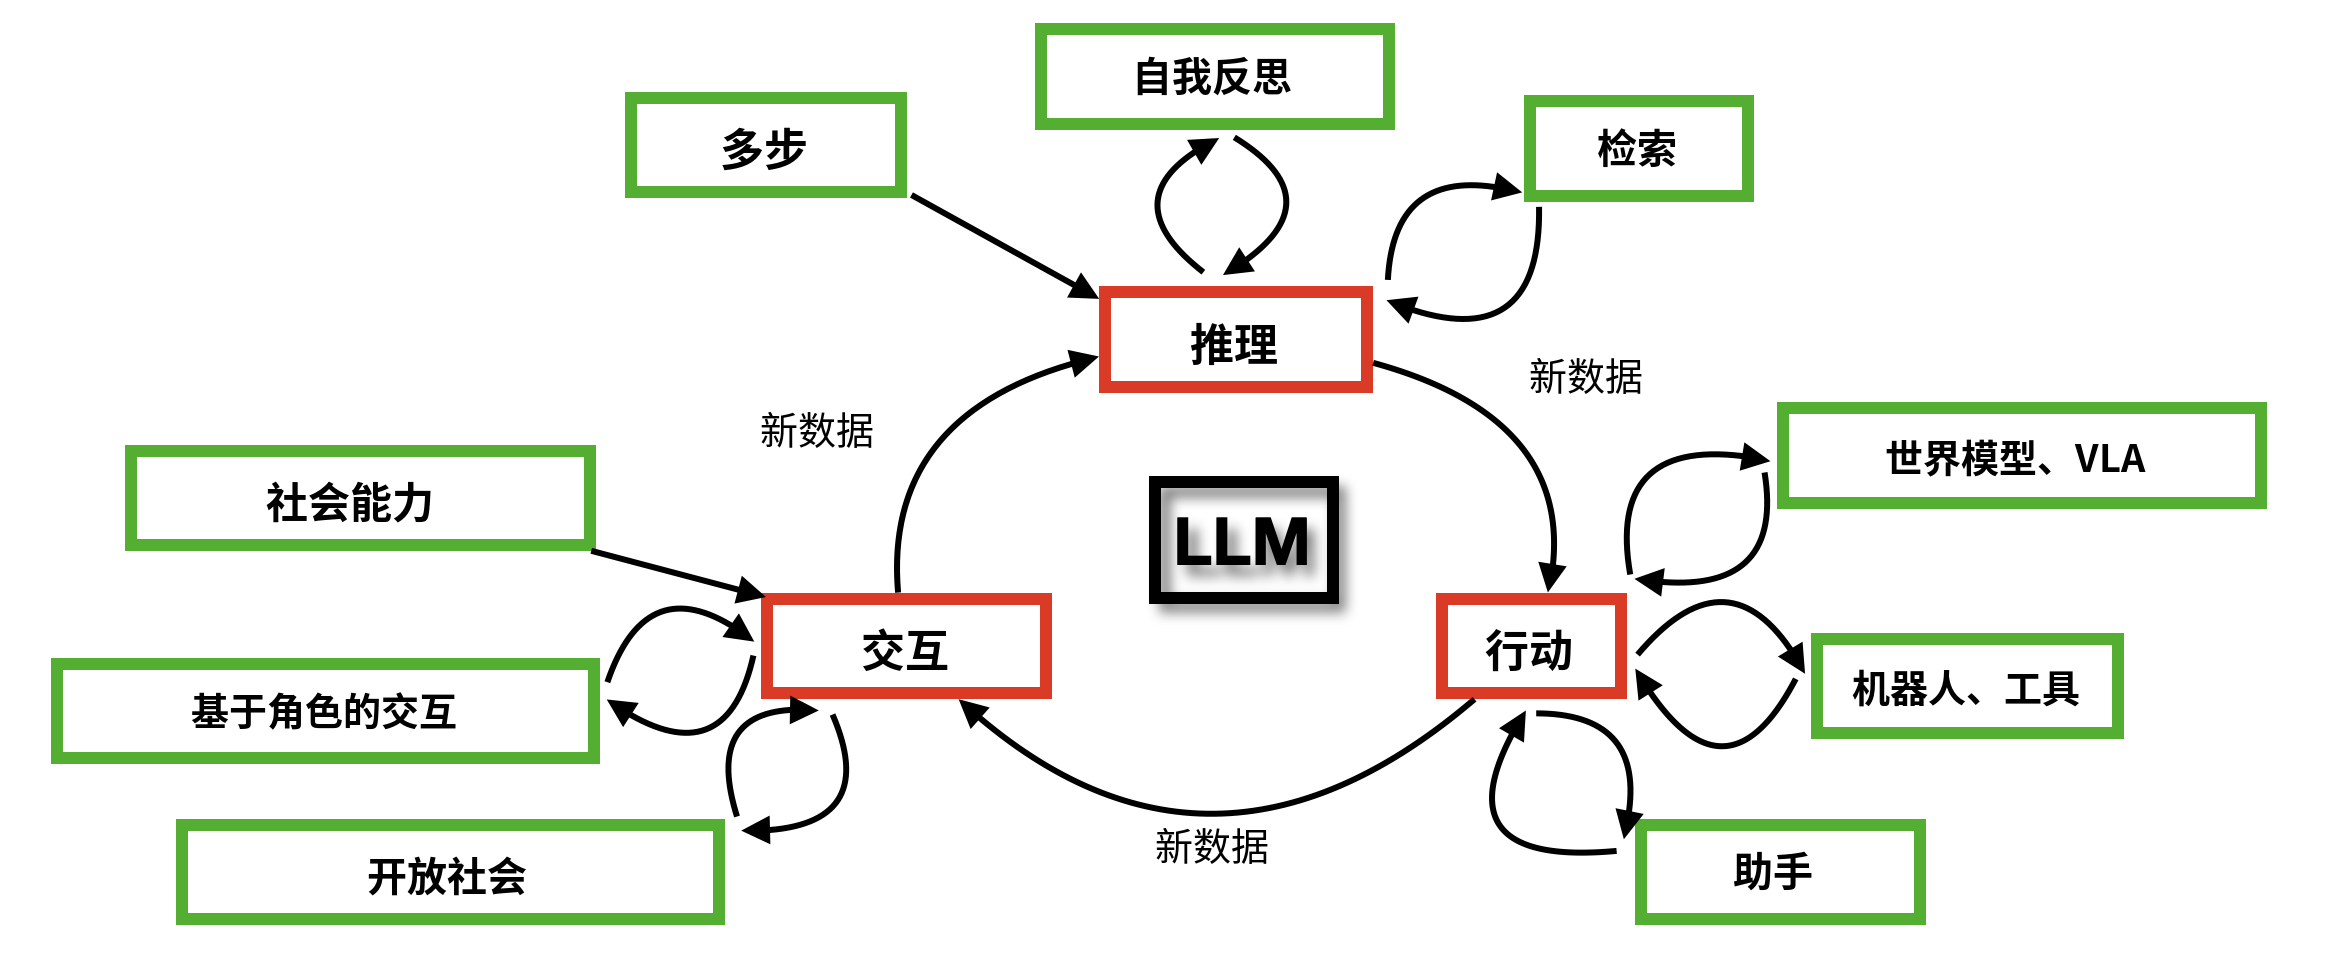
\includegraphics[width=0.75\linewidth]{figures/virtuous5}
    \caption{连接三类智能体大语言模型（推理、行动、交互，红色部分，分别对应第二、三/四、五部分）的递归式自我改进循环。影响某一类别的概念以绿色表示。} %Feedback loops, where reasoning, acting, and interacting generate new LLM training data, are also indicated}
    \label{fig:virtuous}
\end{figure}

% Traditionally, LLMs are trained on large datasets. However, recent datasets are becoming so large that it is getting harder and harder to get fresh, high-quality data.  
% , and it is getting harder to improve datasets further. 
%---the entire internet---
% As a consequence, performance of conventional training methods has been plateauing for a while \citep{sutskever2024}.
这带来两点好处。第一，它为动态的智能体行为创造了灵活性与空间，我们将在第~\ref{chap:meta} 章与第~\ref{chap:agents} 章看到这一点。第二，在几乎整个互联网都已被用作模型预训练数据的时代 \citep{sutskever2024}，生成额外的、相关的、高质量的数据变得很有价值。
通过与世界交互，智能体能够自己生成这类新数据。图~\ref{fig:virtuous} 展示了这一过程。这些交互数据可以用于进一步的训练。
% provided that there is adequate grounding, for example through human or automated validation and filtering \citep{subramaniam2025multiagent}. 

大语言模型基于自身智能体行动进行训练的一个例子，是从机器人动作序列中学习的视觉—语言—动作模型（第~\ref{chap:world} 章）。%\citep{black2024pi_0,chiang2024mobility,yang2025magma}. 
另一个例子见第~\ref{chap:emergent} 章：在那里，智能体社会让模型通过交互变得更聪明，就像人类在彼此交往中学会新的行为与想法一样。

因此，除了催生有用的应用之外，
%that are useful in different applications, 
智能体大语言模型的另一个驱动力，是生成更多训练数据的机会——它构成了一个递归式自我改进循环。图~\ref{fig:virtuous} 展示了这一交互式数据生成的良性循环。图中红色标出的是主要类别：推理（第二部分）、行动（第三/四部分）与交互（第五部分）。绿色标出的是会直接影响某一类别、或通过反馈循环影响某一类别的概念。

% \footnote{Sociology teaches
%   us that humans become more intelligent through interaction with the world and with other humans (we learn new behaviors and ideas from others). Societies of agents allow
%   agentic LLMs to become more intelligent through interaction---as we will see in Section~\ref{sec:interacting}.} %(See Figure~\ref{fig:virtuous}.)

% The emergence of agentic LLMs is driven by progress in natural language processing, reasoning models, tool integration, reinforcement learning, agent-based modeling, and  social science.  %At the confluence of these fields many exciting publications have emerged. 


\section{读者对象与目标}
本书主要面向人工智能与计算机科学方向的研究生与研究者。对来自其他领域的学生与学者（例如认知科学、社会科学或人文学科）也可能有吸引力——只要他们有内在的动力去接触机器学习与技术挑战。

本书的目标是介绍并综述智能体大语言模型领域的技术进展与应用。
我们会较深入地讨论智能体大语言模型工程的主要概念。我们提供科学文献的引用，以及源代码和数据集的链接，方便你自己动手构建智能体。请注意，这个领域很新，而且仍在快速变动之中。扎实理解基础知识，对于跟上最新进展至关重要。我们的目标是把这两者都提供给你。

我们使用本书讲授「智能体大语言模型」课程，它是莱顿大学计算机科学（人工智能方向）与创意智能与技术硕士项目的一部分。配套网站提供了支持材料（讲义幻灯片、作业、新闻）。\footnote{\url{https://agenticllms.liacs.nl}} 

亲爱的读者，我们希望你在阅读本书时获得的乐趣，不亚于我们写作时的乐趣。智能体大语言模型研究是一个新领域，本书同样新鲜。新进展每天都在出现。我们非常欢迎你通过网站，为本书的后续版本提供反馈与建议！

\section{前置知识}
本书假定你具备本科水平的计算机编程、人工智能、机器学习与自然语言处理知识。

我们假定你会使用 Python 与 PyTorch。我们还假定你理解机器学习的原理，例如分类与回归的区别、训练集与测试集的区别，以及过拟合与欠拟合的成因。你应当了解经典机器学习方法，如决策树、集成方法与随机森林。你还应熟悉深度学习的概念，例如人工神经网络的架构（全连接多层感知机、卷积神经网络与循环神经网络）、通过反向传播进行学习，以及损失函数（如交叉熵）与激活函数（如 ReLU）。我们还期望你熟悉强化学习：你应当知道什么是顺序决策问题，理解智能体与环境的区别，并知道如何使用一些策略学习算法（如 Q 学习、DQN、PPO 与 SAC）。最后，你应当对自然语言处理有所了解：什么是分词、什么是词嵌入、什么是注意力，以及什么是 Huggingface。

不过我们也相信，即使你对上述部分或全部主题与概念了解不深，读这本书仍然会有收获。我们对核心主题提供了简要综述，%. Your journey may require some occasional extra study, but  
你将以一个有价值的水平了解智能体大语言模型，并找到进一步学习的切入点。
对其中一些主题，手边有一本合适的教材会很有帮助，\footnote{参见 \citet{gunasekar2024textbooks}}例如：
\begin{itemize}
    \item 
经典机器学习：\citet{alpaydin2021machine,flach2012machine}，
\item 深度监督机器学习：\citet{bishop2023deep,goodfellow2016deep,chollet2021deep,stevens2020deep}，
\item 强化学习：\citet{sutton2018reinforcement,graesser2019foundations,plaat2022deep,franccois2018introduction}，
\item 自然语言处理与 Transformer：\citet{jm3}。
\end{itemize}
%, and have basic knowledge of LLMs (tokenization, embeddings, attention mechanism, transformer architecture).

%A basic understanding of PyTorch, Reinforcement Learning and LLM is expected.

\section{课程结构}
我们使用本书讲授本校的智能体大语言模型研究生课程。本书力求既简明又全面：我们在适合研究生课程的水平上覆盖该领域的完整广度。为了让你能深入钻研，我们提供了大量科学文献的指引，一些进阶主题则放在标有 * 的章节中。

不同高校的项目可能覆盖不同材料（见表~\ref{tab:flow}）。我们讲授的课程内容全面，由 14 讲构成：一次导论课，然后 3 讲讲第一部分（语言建模），3 讲讲第二部分（推理）与第三部分（智能体），3 讲讲第四部分（工具与助手），3 讲讲第五部分（社会模拟）。课程以一次期末评述课收尾。我们的课程把四个案例研究作为作业，通过与学生的面谈来评分。我们在期末没有单独的理论考试，课程成绩取各次作业成绩的平均。

当然，你完全可以按自己情况合理的方式使用本书，但我们主要覆盖智能体大语言模型的两类用例：（1）助手，（2）社会模拟。

如果你的项目另有专门的大语言模型进阶课程，那么以（1）智能体助手为核心的项目可以只包含第二、三、四部分。作业方面，我们建议做案例研究 2 与 3。

或者，以（2）社会模拟为核心的项目应覆盖第二、三部分以及第五部分，作业使用案例研究 2 与 4。

助手路线与社会模拟路线都可以视需要补充第一部分（语言建模），具体取决于你所在高校的培养方案如何设置。

第六部分包含进阶主题。第~\ref{chap:synthetic-data} 章关于合成数据生成，适合「助手」用例（第四部分）。第~\ref{chap:mi} 章关于机制可解释性，适合为第一、二部分（语言模型与推理模型）做更深入的拓展。
第~\ref{chap:arch} 章关于高级架构，也适合第二部分。
第~\ref{chap:cognition} 章关于认知架构，适合「社会模拟」用例（第五部分）。

\begin{table}
    \centering
    \begin{tabular}{l|l|l|l|l}
        课程目标 & 部分 & 案例研究& 章节 & 选读  \\ \hline
        全面 & I, II, III, IV, V & 1, 2, 3, 4 & 1-18 & 19-22\\
        助手核心 & II, III, IV & 2, 3 & 6-14 & 2-5, 19\\
        社会模拟核心 & II, III, V & 2, 4 & 6-10, 11, 15-18 & 2-5, 22\\
    \end{tabular}
    \caption{不同课程目标与本书各部分、各章节的对应关系}
    \label{tab:flow}
\end{table}

表~\ref{tab:flow} 汇总了把本书材料用于三种不同课程目标的各种方案。


\section{方法、范围与全书概览}
我们的方法是动手实践式的。对所有新概念，我们都提供理论背景，并给出在实践中如何使用它们的例子。我们讨论数据集、训练算法、基准测试、训练环境，给出重要智能体算法的伪代码，并提供实践案例研究来帮助你学习。

本书按章组织，每章覆盖一个完整的主题。各章归入七个部分。

第一部分对大语言模型做基础介绍。第~\ref{chap:llm} 章讨论重要的自然语言处理概念，如分词、嵌入、循环神经网络、注意力机制、Transformer 架构，以及自回归训练（这是 LLM 训练方式所依托的核心机器学习方法）。我们还讨论了进一步的机器学习方法：监督学习与强化学习。接着，在第~\ref{chap:pipeline} 章中，我们较详细地讨论用于训练 LLM 的训练流水线。我们讨论数据集的获取、预训练、微调、指令微调、价值对齐与推理。我们还会讨论常用于测试 LLM 性能的基准测试。在第~\ref{chap:scaling} 章中，我们讨论缩放定律与小语言模型，并讨论能耗问题。要能够使用智能体大语言模型，你必须理解预训练与微调 Transformer 模型的基础。在第一部分最后一章中，我们通过一个实践案例研究帮你获得这一经验——我们将引导你从零训练一个 Transformer 模型。

第二部分介绍推理、反思与世界模型这几个概念，它们是（高级）智能体大语言模型的必备要素。%We will see how concepts from reinforcement learning are not only used to finetune LLMs, but also how the agentic LLM itself operates as a reinforcement learning agent in an environment. 
在第~\ref{chap:reasoning} 章中，我们从上下文学习出发，讨论思维链方法如何使 LLM 能够对简单的数学应用题进行多步推理。我们将讨论如何借助运行框架，让 LLM 对自己的上下文学习进行自我反思，以增强其推理能力。到目前为止，我们关注的都是使用语言的模型。要在现实世界中行动，我们的智能体还必须理解图像数据以及其他模态。在第~\ref{chap:world} 章中，我们走出语言，讨论理解视觉与语言的模型，以及从决策序列中学习、知道如何执行机器人动作的模型。要在世界中行动而不撞墙，智能体需要对物理有一定理解。在第~\ref{chap:world} 章中，我们讨论世界模型，包括它们与基于模型的强化学习的关系。
到那时，我们已经讨论了智能体学习和与环境交互的多种不同方式。在第~\ref{chap:meta} 章中，我们将更深入地讨论它们如何学习，以及这种学习为何是一种元学习。

接下来，在第三部分，第~\ref{chap:agents} 章从人工智能的视角对智能体做了历史回顾，并讨论智能体大语言模型的不同交互风格。此外，要在世界中行动，智能体需要某种形式的记忆。我们在该章讨论不同的智能体记忆架构。第三部分以一个实践案例研究收尾，你可以在其中为 BALROG 基准测试套件中那些颇具挑战的谜题与游戏，构建一个能自我反思的智能体。

%Agentic LLMs are an active field of research, where many frameworks have been developed to help you implement your own agent. 
在第四部分，我们换挡：从理论概念转向实践实现。我们讨论社区中为构建智能体大语言模型、以及让它们使用工具在世界中行动而开发的各种框架。有些是专有的，但许多是开源的，可以从 Github 下载。在本部分中，我们讨论为用户行动并完成实际任务的智能体。在第~\ref{sec:tools} 章中，我们讨论为实现智能体大语言模型而开发的工具链、框架与 API。在第~\ref{sec:rag} 章中，我们讨论检索增强方法，以及其他用于搜索「LLM 训练时尚不存在的最新信息」的方法。第~\ref{sec:assist} 章综述智能体大语言模型的实际应用。我们讨论 LLM 的各类应用，如购物助手、医疗助手、交易助手，以及帮助开展科学研究的助手。第四部分最后一章以一个实践案例研究收尾，说明如何构建一个医疗诊断智能体（同时也是为了帮你理解它的短板，从而永远不会盲从一个智能体的医疗建议）。

第五部分采取不同的视角：我们从行为与认知的角度、而非技术的角度来审视智能体大语言模型。在总体界定并介绍机器行为研究之后，第~\ref{chap:behavior} 章讨论在受控的实验情境中测试单个 LLM 与智能体大语言模型的社会行为。第~\ref{chap:role} 章转向多智能体系统，先讨论基于角色的交互——即把智能体大语言模型构建或提示为扮演某种角色，并以目标导向的方式交互。接着，在第~\ref{chap:emergent} 章中，我们转向由多个智能体组成、以开放式方式交互的系统，研究{\em 涌现行为}，例如合作与规范执行。该案例研究让你能够深入体验社会性的智能体行为。

接下来的第六部分包含更进阶的材料。
第~\ref{chap:synthetic-data} 章讨论合成数据生成。与所有形式的深度学习一样，LLM 在很大程度上仍是一个黑箱，我们讨论一些能揭开一角面纱的技术。
第~\ref{chap:arch} 章讨论高级架构。我们讨论在决策轨迹上训练的 Transformer，以及循环式与递归式 LLM。我们还讨论高级智能体架构：上下文强化学习、自修改智能体与元智能体。
第~\ref{chap:mi} 章聚焦于机制可解释性工具，用于刻画 Transformer 架构中神经元活动的模式，从而更好地理解 LLM 的推理过程。%The chapter %~\ref{chap:black} 
%discusses methods from explainable machine learning.
在第~\ref{chap:cognition} 章中，我们综述关于智能体大语言模型行为与认知的最新文献，包括关于心理理论与意识的进阶问题。

最后，在第七部分中，我们把本书所提供的智能体大语言模型各个要素汇总起来。在第~\ref{chap:concl} 章中，我们讨论智能体大语言模型目前能做什么、仍然做不到什么，并以对未来可能带来什么的展望收尾。

% We use this book for a full semester course in the Master Program Computer Science at our university. 
请注意，部分章节标有 *。这些章节包含更进阶的材料，可能更适合写论文而非课程学习。

\section{致谢}
本书源于我们对智能体大语言模型的热忱——这份热忱带来了与许多学生和同事的讨论，也带来了令人兴奋的研究。到某个时刻，我们觉得自己必须写出这本书、并开设一门研究生课程。我们相信，智能体大语言模型是一个极其重要的主题，许多 AI 方向的学生都会想了解它。

本书中的部分材料基于并受惠于早期工作（例如参见 \citet{van2023theory,van2024hybrid,huisman2021survey,moerland2023model,plaat2022deep,plaat2024reasoning, plaat2025agentic,van2024llamea,chen2025does,van2025baba,xing2025cocomposer}）。我们感谢这些工作的所有合著者——没有你们，这本书不可能写成！

第 \ref{chap:generative_agents} 章中关于生成式智能体社会的案例研究，由 Dorota Moravčiková 与 Friso van der Veen 撰写并开发（基于 \citep{park2023generative}），他们把自己在这个主题上的已有工作改写以适配本书。我们也感谢他们慷慨的付出以及对前几章提出的犀利意见。

我们感谢本研究所的学生与同事。特别感谢 Thomas B\"ack、Joost Batenburg、Joost Broekens、Xi Chen、Lennard Froma、Bas Haring、Anna Kononova、Tom van Kouwenhoven、Thomas Moerland、Rob van Nieuwpoort、Mike Preuss、Peter van der Putten、Zhaochun Ren、Derya Soydaner、Suzan Verberne、Fien van Wetten、Annie Wong 与 Tarik Začiragić，感谢他们许多富有成果的讨论。

\bibliographystyle{plainnat}
\bibliography{agenticbook,refs,case,synthetic}
